\chapter{ODOO PLM 簡介}
\renewcommand{\baselinestretch}{10.0} %設定行距
%\pagenumbering{arabic} %設定頁號阿拉伯數字




\fontsize{14pt}{2.5pt}\sectionef\hspace{12pt}


Odoo 產品生命週期管理(PLM)模組可以幫助企業對於產品的生命週期管理:從客戶需求→設計開發→產品測試→大量生產→產品維護→產品停產下架,PLM模組中可以為這個工作項目指派負責人員以及完成所需時間,負責這個項目的人員就可以對進度進行提交、修改,或是提出時間延長讓項目有更充裕的時間完成,每次項目提交都會以歷史紀錄保存,方便團隊追溯產品的修改紀錄。\\




\begin{figure}[h!]
\begin{center}
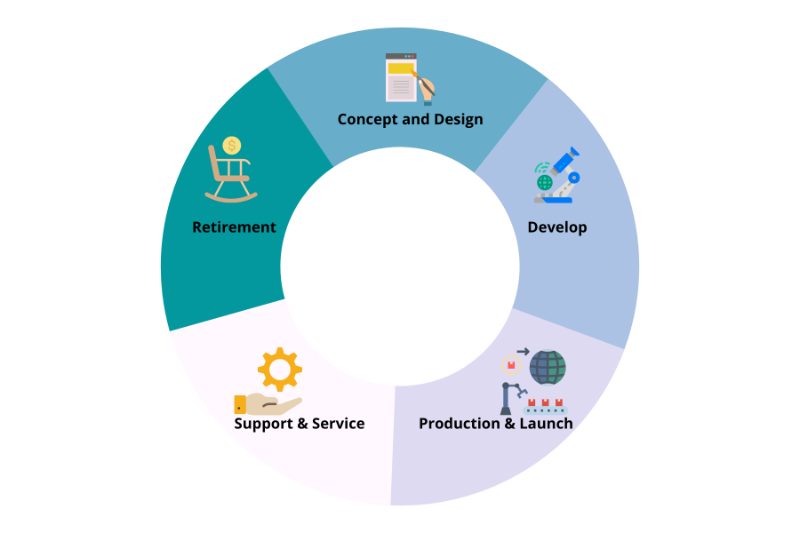
\includegraphics[width=12cm]{PLM_structure}
\caption{\large PLM structure}
\label{PLM_structure}
\end{center}
\end{figure}









\newpage

\renewcommand{\baselinestretch}{0.5} %設定行距